\chapter{介绍}
近年来,以神经网络\upcite{alexnet2012}为代表的深度学习方法在图像处理\upcite{vgg2014, inception2015, resnet2016, denselynet2017}、机器视觉\upcite{rcnn2014, fastrcnn2015, fasterrcnn2015, yolo2016, fpn2017, rfcn2016}、自然语言处理\upcite{gnmt2016, bert2018}等诸多应用领域取得了巨大突破。随着神经网络的不断发展以及社会对人工智能应用需求的提升,深度学习所需的数据量、网络模型也越来越大,单台计算机算力已经很难甚至无法满足其计算要求。为了减少神经网络的训练时间和适应不断增长的算力要求,分布式训练神经网络是必然选择。

目前分布式通信框架主要有parameter servers\upcite{ps2014}和horovod\upcite{horovod2018},主流的深度学习框架均支持这两种通信框架。如tensorflow,pytorch,mxnet等\upcite{tensorflow2016, torch2002, mxnet2015}。
parameter servers最早由smola教授提出,最终由其学生李沐实现。其提供同步、异步、半异步的更新方式,因其灵活的更新方式和良好的性能得到业界广泛认可。参数服务器通过key-value键值对来管理参数。通常情况下,参数服务器是以去中心化的形式分散在多个节点,各个节点负责部分数据的同步。horovod\upcite{horovod2018}是uber基于百度ring-allredue的通信方式,提出的分布式通信框架,因为其优异的性能和简单的使用方式,在业界引起广泛关注。horovod基于MPI实现,为提高分布式通信的效率,提出tensor fusion和分层级同步策略等方法,极大提高了分布式训练效率。 

二者均从网络通信方式,数据组织形式等方面对通信效率进行了优化,确没有针对神经网络训练特点进行相关优化。根据目前业界对低精度数据在神经网络中的研究现状可知,低精度数据(如BF16和FP16)在一定优化方法下均能保证神经网络的精度。本文针对神经网络对数据精度要求不高的特点,提出低精度分布式更新(LPDU)算法,算法主要包含两部分:低精度数据通信和混合精度更新。算法核心思想是把原始浮点数梯度转换为BF16格式的低精度数据进行全局同步,使得同步数据量减半,进而减小同步时间开销,提高分布式训练效率。同时为保证神经网络的训练精度,本文使用混合精度更新算法对神经网络进行更新。

现阶段神经网络均采用严格同步方式进行训练,基于allreduce的horovod的通信效率略高于parameter servers,故本文所有算法均基于horovod实现。

\chapter{相关工作}
随着网络模型的不断增大,数据日益增加以及应用需求的剧增,在深度学习发展历程中,分布式训练神经网络是必不可少的一环。目前主要有数据并行和模型并行两种方法用于分布式训练,如图\ref{fig:data_model_parallel}所示。

\begin{figure}[htp]
\centering
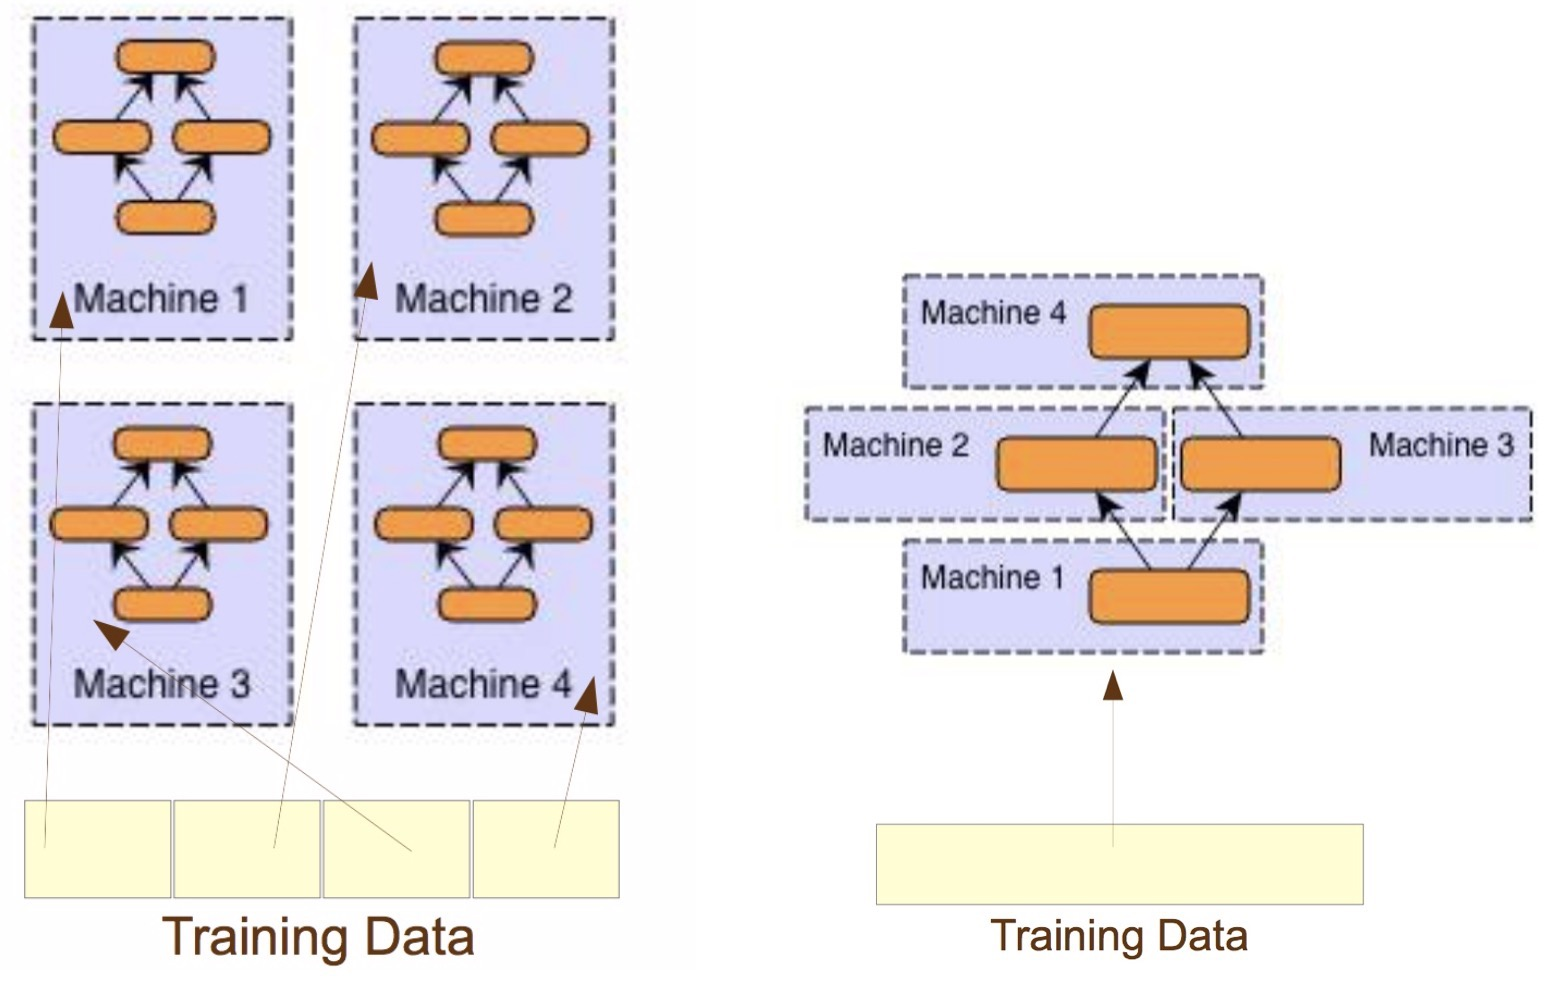
\includegraphics[width=13cm]{data_model_parallel}
\caption{数据并行(左)与模型并行(右)示意图}
\label{fig:data_model_parallel}
\end{figure}
数据并行是把数据分到不同的计算节点上,让不同节点处理不同的数据。因为有多个节点在并行地处理数据,所以在单位时间内,理应能够处理更多的数据,也即达到了并行计算的目的。在数据并行模式下,每个节点都会保留一份完整的网络模型和参数$w^{j}$,在严格同步下,通信主要包含两部分:对本地梯度数据求和,广播全局更新后的参数$w^{j}$到各个节点。在第一步,每个节点都将发送本地梯度$\nabla w^{j}$到管理节点,当管理节点收到所有节点梯度$\nabla w^{j}$时,将对参数进行更新,如公式~\ref{equ:dp_update}所示;第二步管理节点将把全局更新后的$\widetilde w$广播至所有计算节点。目前绝大部分神经网络均通过数据并行方式进行分布式训练。
\begin{equation}
\label{equ:dp_update}
\widetilde w \leftarrow \widetilde w - \eta /P \sum^{P}_{j=1}\nabla w^{j}
\end{equation}


模型并行则是把一个大的网络模型划分成很多小块,然后把每小块对应的参数、状态和计算任务分到不同的计算节点上执行,类似于流水线作业。模型并行除了通过模型并行获得加速外,当某些模型在单机上无法训练的时候(如内存不够),则只能通过模型并行才能完成训练。目前业界绝大部分训练以数据并行的方式进行训练。

即随着分布式规模不断增大,在数据并行方法下必然导致用于训练的神经网络的batch size线性增大,在大batch size情况下,如何保证单机batch size相同的精度是分布式深度学习中重要难题。尤其是在分布式规模较大情况下,传统SGD更新算法已经无法保证训练精度,需要新的更新算法保证网络精度。如facebook提出的热启动、线性增大学习率方法\upcite{train1hour2017},在保证训练精度情况下,将batch size提升至8k;线性增大学习率是指:当batch size从$B$增大到$kB$时,此时学习率也要由$\eta$增大至$k\eta$;热启动则表示:学习率$\eta$应逐渐增大至$k\eta$,假设热启动的迭代次数为$I$,则在第$i$次迭代中学习率为$\eta _{i}=\eta + i(k-1)\eta/I$。随后用伯克利的尤洋等\upcite{train24min2017}提出的分层自适应学习率的方法,进一步将batch size提升至32k;其核心思想是每个网络层参数及其梯度数值差距很大,不应使用相同学习率$\gamma$对其进行更新,而应设置不同学习率分别更新对应参数。其学习率计算如公式~\ref{equ:lars}所示。进一步谷歌大脑\upcite{dontdecay2018}提出通过逐渐增大batch size替换学习率衰减的方法,最终将batch size提升至64k,只用两千五百多次迭代将ImageNet训到了理想精度。
\begin{equation}
\eta = l \times \gamma \times \frac{||w||_{2}}{||\nabla w||_{2}}
\label{equ:lars}
\end{equation}

由于神经网络本身存在随机性和容错性的特点,其计算精度并不需要达到浮点数的精度,为了节省内存,带宽,以及在支持低精度计算的硬件设备上提升计算效率,业界提出了两种主流的低精度数据格式用于神经网络训练。分别是IEEE半精度浮点数(FP16)和bfloat16(BF16)格式。两者与浮点数据格式区别如表~\ref{tab:diff_format_bits}所示。

\begin{table}[htbp]
\centering
\begin{minipage}[t]{0.9\linewidth}
\caption{不同数据格式比特位的分布}
\label{tab:diff_format_bits}
\begin{tabularx}{\linewidth}{l X X X X}
\toprule[1.5pt]
{\song 数据格式} & {\song 总比特位数} & {\song 符号位数} & {\song 指数位数} & {	\song 尾数位数}\\
\midrule[1pt]
FP32 & 32 & 1 & 8 & 23\\
FP16 & 16 & 1 & 5 & 10\\
BF16 & 16 & 1 & 8 & 7\\
\bottomrule[1.5pt]
\end{tabularx}
\end{minipage}
\end{table}
由科学计数法可知,表~\ref{tab:diff_format_bits}中3种数据格式在不同指数情况下,精度范围有所不同,3种数据格式所能表示的最小精度如表~\ref{tab:diff_format_precision}所示。经过工业界验证,这两种低精度数据格式均保证神经网络的收敛精度,逐渐成为主流。目前主流的深度学习框架tensorflow,pytorch,MXNet均支持半精度浮点数计算,BF16数据格式目前只有tensorflow针对自家硬件TPU有所支撑。

\begin{table}[htb]
\centering
\noindent\begin{minipage}{0.5\textwidth}
\centering
\caption{不同数据格式数据精度和有效数字位}
\label{tab:diff_format_precision}
\begin{tabular}{p{2cm}p{2cm}p{3.5cm}}
\toprule[1.5pt]
数据格式 & 数据精度 & 有效数字位(十进制)\\\midrule[1pt]
FP32 & 0.00000012 & 6~7\\
FP16 & 0.00097656 & 3~4\\
BF16 & 0.00781250 & 2~3 \\
\midrule[1pt]
\end{tabular}
\end{minipage}
\end{table}
2017年Micikevicius P等为节省训练的内存开销,提出混合精度训练\upcite{mixed2018}的方法,使用IEEE半精度格式存储所有网络层的中间结果。相对于原始32位浮点数计算而言,训练网络模型所消耗的内存减小了一半;同时,为了弥补半精度表示所带来的损失,文章提出混合精度训练的方法。在设计损失函数时,适当放大损失函数权重的方法来保证训练精度。

\chapter{算法设计}

本章将详细介绍本文提出的低精度分布式更新(LPDU)算法,主要分为两部分:低精度数据通信(LPDC)算法和混合精度更新(MPU)算法。同时还将介绍分别适用于不同任务场景的精度梯度压缩(EPGC)算法的实现原理。

\begin{figure}[htp]
\centering
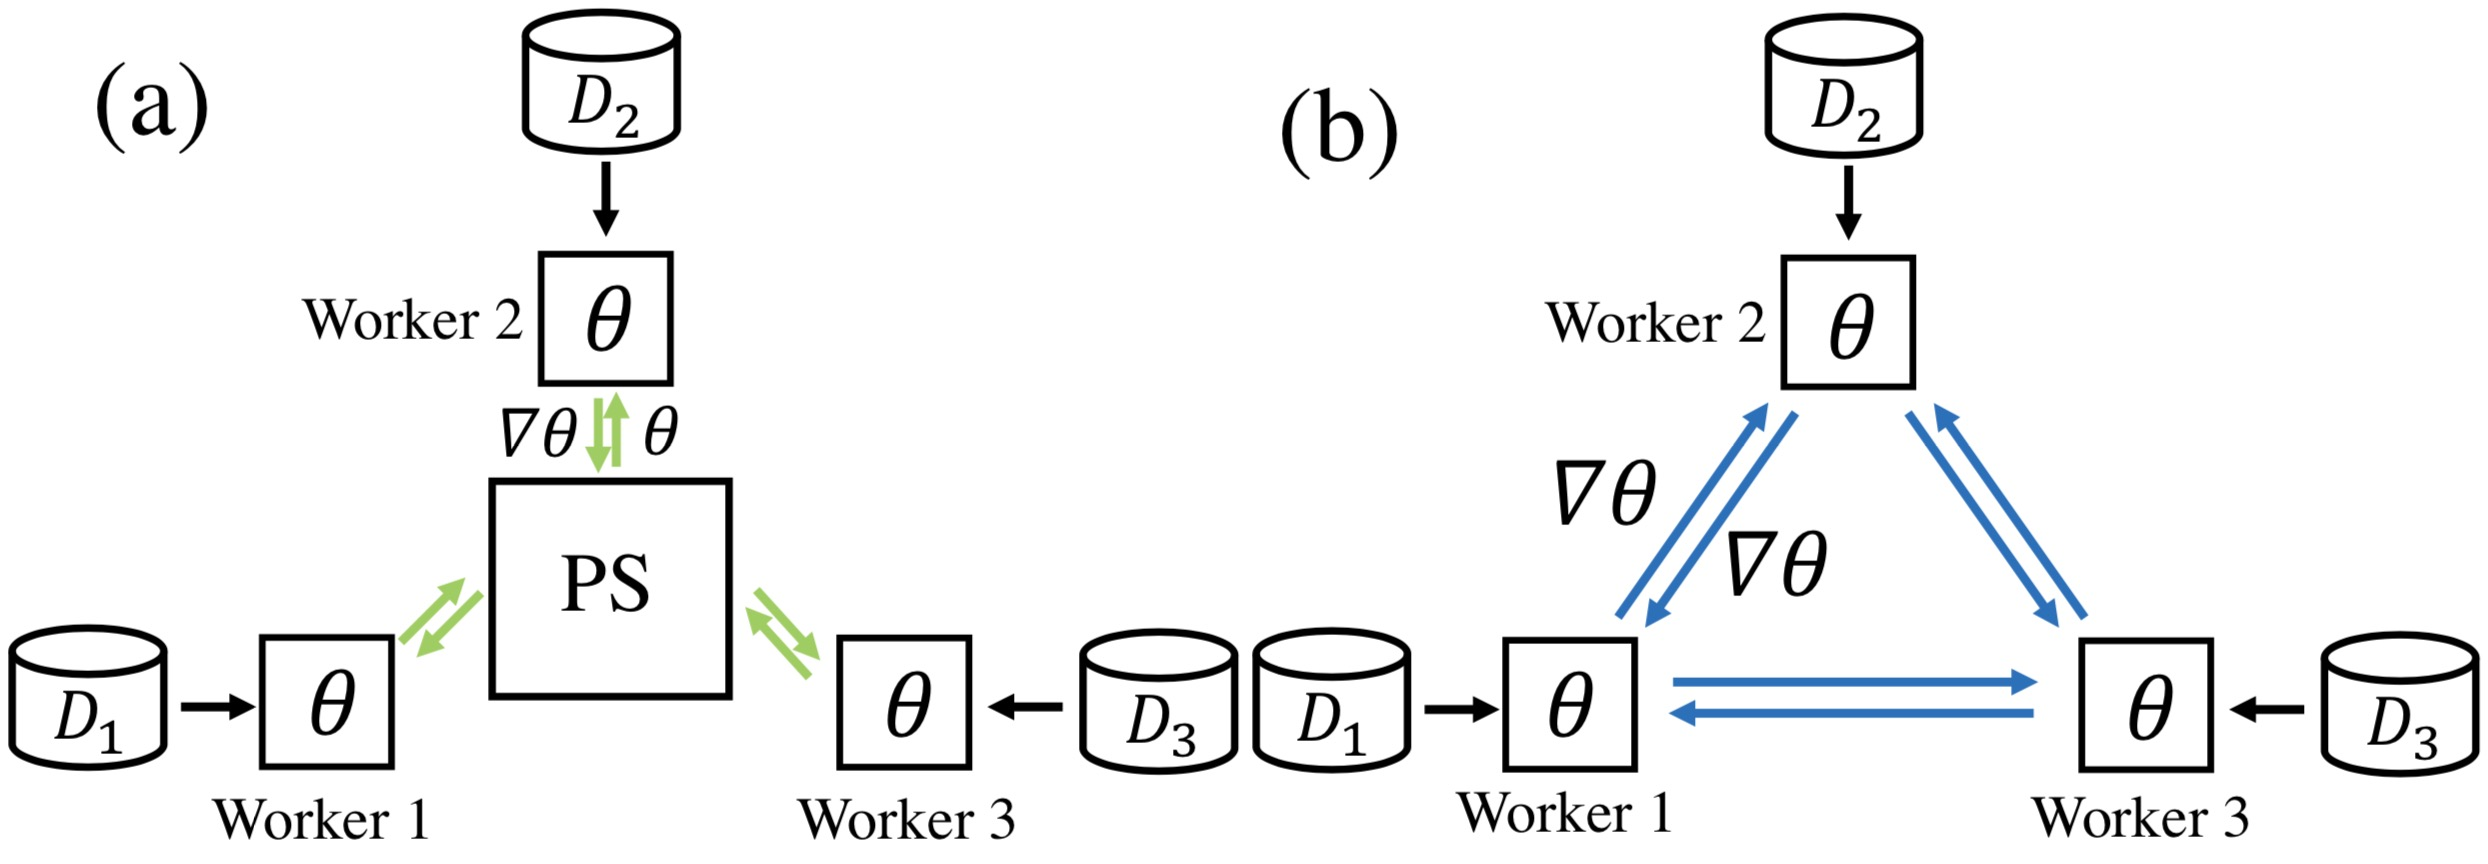
\includegraphics[width=13cm]{ps_allreduce}
\caption{PS(a)和MPI(b)下数据并行的实现原理}
\label{fig:ps_allreduce}
\end{figure}

在数学形式上,给定数据集$D$,损失函数$L$,拟合参数为$\theta$的神经网络的过程,可以被建模成公式~\ref{equ:nn_equ}形式。其中$t$表示迭代次数,$\nabla L$表示在当前参数$\theta^{(t-1)}$,数据为$D^{(t)}\subset D$,学习率为$\epsilon$时,损失函数的梯度。在不断迭代过程中,直至$\theta$达到终止要求。
\begin{equation}
\label{equ:nn_equ}
\theta^{(t)}=\theta^{(t-1)}+\varepsilon\cdot\nabla L(\theta^{(t-1)},D^{(t)})
\end{equation}

在分布式深度学习中,通常采用数据并行的方式进行分布式训练,其通过将数据集$D$划分,放在不同计算节点(下标为$p=1,...,P$)上,如图~\ref{fig:ps_allreduce}所示。在每次迭代$t$中,每个计算节点从各自数据集$D_{p}$获取单次迭代数据$D^{(t)}_{p}$,并计算模型梯度$\nabla L(\theta^{(t)},D^{(t)}_{p})$;随后系统将各个节点梯度进行聚合,使用下列公式~\ref{equ:nn_dl_equ}对模型进行更新。
\begin{equation}
\label{equ:nn_dl_equ}
\theta^{(t)}=\theta^{(t-1)}+\varepsilon\sum^{P}_{p=1}\nabla L(\theta^{(t-1)},D^{(t)}_{p})
\end{equation}

在数据并行模式下,每个计算节点都要在本地维护一份全局共享参数$\theta$,这将产生大量的通信开销。目前主要有参数服务器(图~\ref{fig:ps_allreduce}a)和MPI(图~\ref{fig:ps_allreduce}b)两种方法来实现全局参数的维护。本文算法则是基于MPI通信模式提出。假设神经网络模型参数$\theta$的数据量为$M$,由图~\ref{fig:ps_allreduce}b可知,在每次迭代$t$中,每个worker会发送、接受模型当前梯度$\nabla\theta$,其大小与模型参数$\theta$相同,即每个worker都会产生$2M$的通信数据量。该通信数据量大小对分布式训练神经网络的效率影响至关重要。本文提出的LPDU算法针对神经网络自身的容错性及其对数据精度不敏感的特点,将32比特浮点数表示的梯度数据$\nabla\theta$转换成16比特的bfloat16数据格式,使得$\nabla\theta$的数据量由$M$减少至$M/2$。此时,每次迭代$t$中每个worker传输的数据量从$2M$减少至$M$,使得分布式系统的通信开销降低,提升系统训练效率。且神经网络参数$\theta$的数据量越大,提升效果越明显。

LPDU算法主要包含两部分:低精度数据通信和混合精度更新。低精度数据通信部分旨在减少分布式训练过程中的同步通信开销,从而提升分布式训练效率;混合精度更新部分则是为避免低精度数据表示带来的数据精度损失造成神经网络训练精度下降的问题,将同步后的低精度梯度数据转换为原始浮点数,再对网络进行更新,可减小更新过程中的数据损失。使用该方法可保证在低精度数据通信情况下神经网络训练精度达到原始浮点数训练的相同精度。

\section{低精度数据通信算法}
由前文可知,相对于单机训练,分布式训练多了额外的同步通信开销,其对分布式训练效率的高低有至关重要的影响。结合业界对低精度数据在神经网络中的研究进展,本文提出一种高效的低精度数据通信方法,在混合精度更新算法配合下,能在不损失神经网络训练精度的情况下,提升分布式训练效率。

算法核心思路是:使用低精度数据进行通信,相对于浮点数通信减少了一半数据量,从而提升训练效率。根据业界对低精度数据在神经网络中的研究进展可知,目前主要有两种低精度数据格式用于神经网络训练,分别是半精度浮点数(FP16)和bfloat16(BF16)数据格式。这两种数据格式在表示数值范围和精度上均有不同程度的损失,通过对应的改进方法,可保证低精度数据下神经网络的训练精度达到原始浮点数训练相同精度。

考虑到FP16与BF16数据格式的特点,BF16数据格式与浮点数之间的转换开销较小;且其可表示的数值范围与浮点数基本相同,故不需要考虑FP16表示情况下梯度数据超过数值表示范围的问题。基于以上两种原因,LPDU算法采用BF16格式数据进行通信,算法内容如算法~\ref{alg:lpdc_alg}所示。

\begin{algorithm}\small
\caption{低精度数据通信算法LPDC}
\textbf{输入:}
浮点数数据:$Data_{fp32}$ \\
\textbf{输出:} 
全局同步后的低精度数据:$Data_{bf16}$
\begin{algorithmic}[1]
	\STATE{将原始32比特的浮点数$Data_{fp32}$转换为BF16格式的低精度数据$Data_{bf16}$}
    \STATE{使用$allreduce$对$Data_{bf16}$做全局同步}
    \STATE{返回全局同步后的低精度数据$Data_{bf16}$}
\end{algorithmic}
	\label{alg:lpdc_alg}
\end{algorithm}

基于BF16格式的低精度数据通信算法的实现主要包含两部分:1.在进行同步之前将原始浮点数转换成BF16格式数据;2.对BF16格式的梯度数据进行同步,求得全局梯度。本文在horovod基础上对低精度数据通信算法进行实现,具体工作包括:1.继承horovod提供的Tensor类,设计BF16 Tensor,供horovod调用,其需要完成原始浮点数到BF16格式数据的转换工作;2.扩展MPI,使其支持BF16格式数据同步,实现一个自定义的BF16求和函数,供MPI在allreduce过程中对BF16数据求和使用。

\section{混合精度更新算法}

由表~\ref{tab:diff_format_precision}可知,BF16格式数据有效数字仅有2~3位,相对于FP32格式数据存在一定精度损失。由随机梯度下降(SGD)更新算法公式~\ref{equ:sgd}可知,SGD将当前梯度乘以学习率$\eta$,再将值更新到模型参数$W$中。通常情况下$\eta$是一个小于1的数,并随着训练的进行,学习率$\eta$逐渐减少。若将$\eta*g_{t,i}$存放在BF16数据格式中,该过程将造成一定的精度损失,产生计算误差,最终该误差将传播到模型参数中。
\begin{equation}
\label{equ:sgd}
W_{t+1,i}=W_{t,i}-\eta*g_{t,i}
\end{equation}

为避免更新过程中产生的精度损失,本文借鉴半精度浮点数训练神经网络的方法\upcite{mixed2018},使用混合精度更新算法来对模型进行更新。如算法~\ref{alg:mpu_alg}所示。其核心思想是:在更新之前将BF16格式梯度数据转换成浮点数据格式,再使用浮点数梯度对网络模型进行更新,从而避免更新过程中产生的精度损失。该算法主要分为两部分:全局同步后的BF16格式梯度到浮点数的转换和SGD算法更新。

\begin{algorithm}\small
\caption{混合精度更新算法MPU}
\textbf{输入:}
本地网络层浮点参数:$Weight_{fp32}$,全局同步后的低精度梯度:$gradient_{bf16}$ \\
\textbf{输出:} 
更新后的网络层浮点参数:$Weight_{fp32}$
\begin{algorithmic}[1]
    \STATE{将全局同步后的低精度梯度$gradient_{bf16}$转换为32比特的浮点数梯度$gradient_{fp32}$}
    \STATE{使用更新算法(如随机梯度下降算法),把转换后的浮点梯度$gradient_{fp32}$更新到网络层参数$Weight_{fp32}$中}
    \STATE{返回更新后的参数$Weight_{fp32}$用于下一次迭代训练}
\end{algorithmic}
	\label{alg:mpu_alg}
\end{algorithm}

同理,混合精度更新算法也适用于带动量的SGD,Adagrad,RMSprop等。实验证明混合精度更新算法能够保证在低精度数据通信方式下,神经网络的训练精度达到原始浮点数训练相同精度。

由上面内容可知,LPDU算法主要包括两部分:低精度数据通信和混合精度更新算法。基于BF16格式数据的LPDU算法如算法~\ref{alg:bf16_update}所示。

\begin{algorithm}\small
\caption{低精度分布式更新算法LPDU}
\textbf{输入:}
本地网络层参数:$Weight$,梯度:$gradient$ \\
\textbf{输出:} 
全局更新后的网络层参数:$Weight$
\begin{algorithmic}[1]
	\STATE{使用LPDC算法求得全局同步后的梯度$gradient_{bf16}$}
    \STATE{使用MPU算法将$gradient_{bf16}$更新到网络层参数$Weight$中}
    \STATE{返回全局更新后的参数$Weight$用于下一次迭代训练}
\end{algorithmic}
	\label{alg:bf16_update}
\end{algorithm}

首先使用LPDC算法完成全局梯度数据的同步,其中通过将原始浮点数据转换为BF16格式数据,在损失部分数据精度情况下减少同步时间开销,以提升分布式训练效率;为避免全局同步后的低精度梯度数据带来的精度损失在更新过程中进一步传播,本文使用MPU算法对模型参数进行更新。LPDU算法下,分布式训练神经网络流程如图~\ref{fig:LPDUflow}所示。实验证明本文提出的低精度分布式更新算法,可在保证神经网络训练精度的前提下,减少分布式训练过程中的同步开销,提升神经网络的训练效率。相关实验结果将在后面详细分析介绍。

\begin{figure}[htp]
\centering
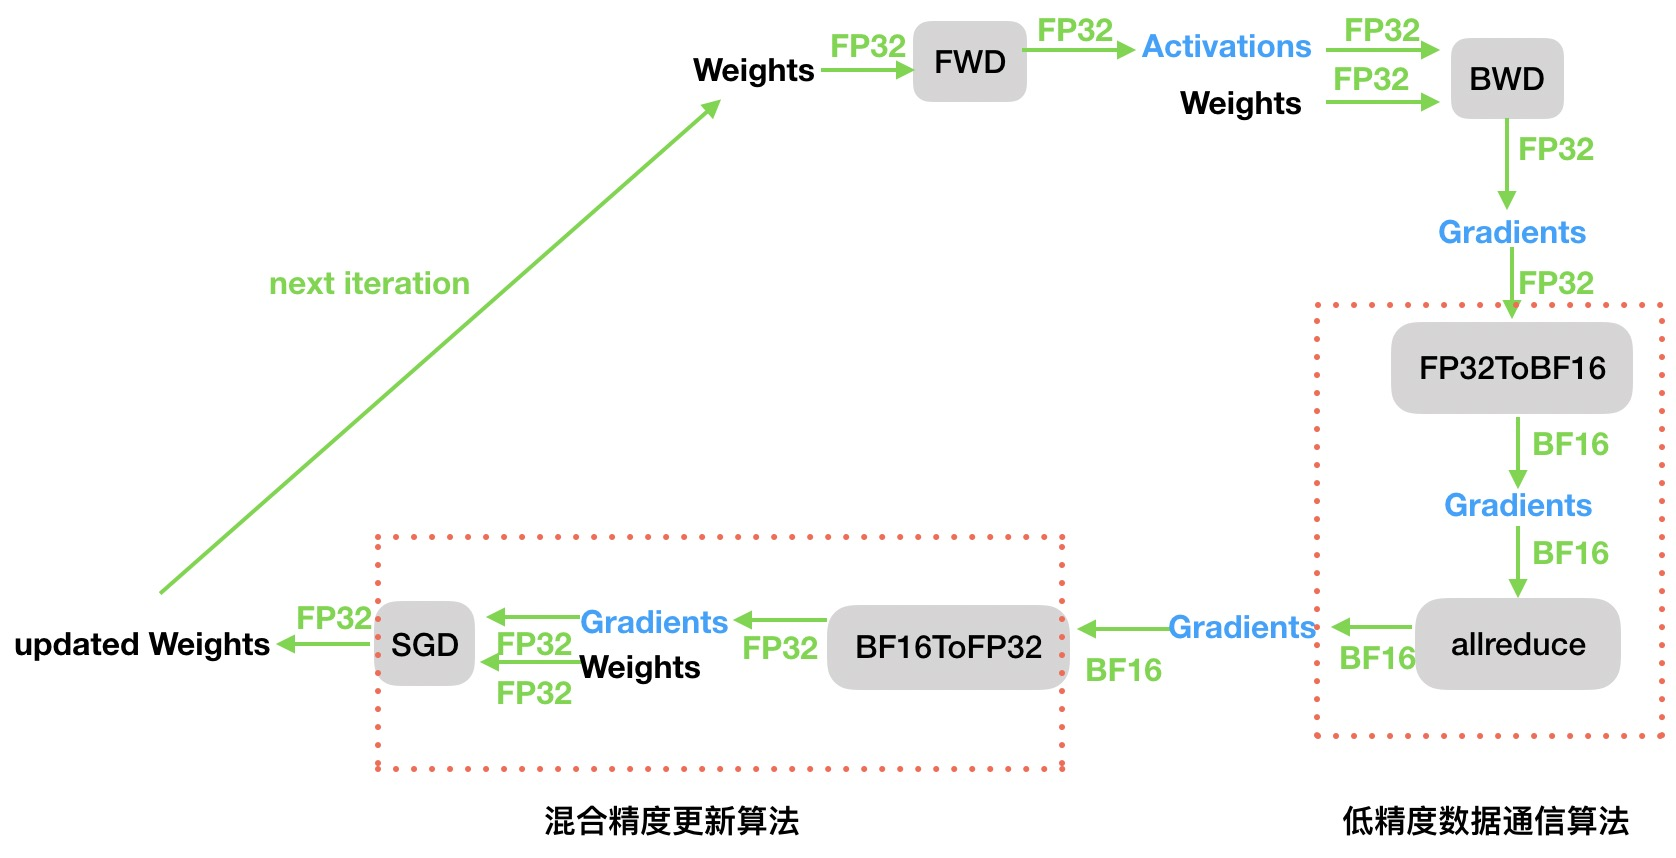
\includegraphics[width=13cm]{LPDUflow}
\caption{低精度分布式更新算法下训练流程图}
\label{fig:LPDUflow}
\end{figure}

\chapter{实验}

在这部分,我们将详细介绍LPDU算法相关的实验以说明算法在不影响神经网络训练精度的前提下对分布式训练效率的提升效果,并介绍2种极限精度梯度压缩方法分别在图像分类和物体检测任务中的训练精度,证明本文提出的2种极限精度梯度压缩方法的可行性。

实验使用的软件主要有:MXNet 1.3版本,OpenMPI 4.0以及开源框架horovod。本文LPDU算法是在ctcyang/horovod:mxnet feature fp16分支基础上进一步设计实现。所有实验结果均是在双sockets的Xeon Gold 6148处理器的集群中运行所得,其中集群网络环境为10Gb以太网。因为目前各个框架CPU端计算性能均基于单socket进行优化。在每个socket上跑一个训练实例可使训练效率达到最佳。故本文在每个机器节点上跑两个训练实例,使得每个socket上跑一个训练实例,以充分发挥CPU计算性能。

\section{LPDU算法效率实验}
为比较LPDU算法与原始更新算法下分布式训练神经网络的效率,本文以Resnet50和SSD网络为例,在真实训练场景中对比LPDU算法与原始算法的效率差异。
为说明LPDU算法相对原始更新算法能够减少同步时间开销,本文以Resnet50为例,在真实训练场景中测得LPDU算法与原始更新算法在不同训练实例个数下的更新时间如表~\ref{tab:fp32_bf16_real_update_time}所示。在8节点16实例情况下,LPDU算法相对于原始更新算法的更新时间有1.3倍的性能提升,在8节点情况下同步时间由原始的0.458s降低至0.352s,可节省30\%的更新时间。 

\begin{table}[htbp]
  \centering
  \caption{不同训练实例中两种算法更新时间}
  \label{tab:fp32_bf16_real_update_time}
  \begin{minipage}[t]{0.8\textwidth} 
    \begin{tabularx}{\linewidth}{|l|X|X|X|X|}
      \hline
      节点数 & 实例数 & origin alg(s) & LPDU alg(s) & Speedup\\
      \hline
1 & 1 & 0.015 & 0.041 & 0.366 \\
1 & 2 & 0.075 & 0.076 & 0.987 \\
2 & 4 & 0.374 & 0.299 & 1.251 \\
4 & 8 & 0.428 & 0.337 & 1.270 \\
8 & 16 & 0.458 & 0.352 & 1.301 \\
      \hline
    \end{tabularx}\\[2pt]
    \footnotesize
    说明:每个实例配置均为resnet50, batch size=128\\
  \end{minipage}
\end{table}

为进一步比较原始更新算法与LPDU算法在实际训练过程中的性能差异,本节通过采样得到不同训练实例下,实际训练中每次迭代时间如表~\ref{tab:fp32_bf16_real_iter_time}所示。可知在8节点16训练实例情况下,LPDU算法的单次迭代时间相对于原始更新算法减少了0.12s,其来自于BF16算法同步时间的降低。该时间与表~\ref{tab:fp32_bf16_real_update_time}中同步时间减少部分相一致。因为LPDU算法降低了同步时间开销,使得分布式训练效率相对于原始更新算法有所提升。如在8节点16训练实例情况下,LPDU算法使得分布式训练效率由84.05\%提升至87.5\%,提升了3.5个百分点。不可否认,现阶段CPU训练神经网络速度远慢于GPU训练,使得分布式训练中通信压力相对较小。若使用GPU训练,单次迭代中计算时间将大大减少,使得同步时间占比增大。此时LPDU算法对提升分布式训练效率的作用将更加明显。

\begin{table}[htbp]
  \centering
  \caption{不同训练实例中两种算法迭代时间}
  \label{tab:fp32_bf16_real_iter_time}
  \begin{minipage}[t]{0.9\textwidth} 
    \begin{tabularx}{\linewidth}{|l|X|X|X|X|X|}
      \hline
      节点数 & 实例数 & origin time & LPDU time & origin & LPDU \\
       &  & (s/iter) & (s/iter) & scaling & scaling\\
      \hline
1 & 1 & 2.8158 & 2.8271 & 100.00 & 100.00 \\
1 & 2 & 2.8685 & 2.9990 & 98.16 & 94.27 \\
2 & 4 & 3.0450 & 3.0387 & 92.47 & 93.04 \\
4 & 8 & 3.3332 & 3.1877 & 84.48 & 88.69 \\
8 & 16 & 3.3501 & 3.2310 & 84.05 & 87.50 \\
      \hline
    \end{tabularx}\\[2pt]
    \footnotesize
    说明:每个实例配置均为resnet50, batch size=128\\
  \end{minipage}
\end{table}

由上述分析可知,神经网络的参数量越大,受网络带宽限制,同步开销越大,LPDU算法对分布式性能提升作用越大。同时,该算法普遍适用于各种主流神经网络,如图像分类,物体检测和循环神经网络等。表~\ref{tab:ssd_vgg_scaling}分别展示了LPDU算法在物体检测网络SSD和分类网VGG中的性能提升。可知模型稍小的SSD网络中,LPDU算法可使分布式训练效率由85.01\%提升至89.84\%,相对于原始更新算法提升了4.83个百分点;在模型较大的VGG网络中该算法性能提升更加明显,相对于原始更新算法,在8节点16训练实例情况下提升了7.13\%。
\begin{table}[htbp]
  \centering
  \caption{原始更新算法与BF16更新算法在SSD与VGG网络中的性能加速}
  \label{tab:ssd_vgg_scaling}
  \begin{minipage}[t]{0.8\textwidth} 
    \begin{tabularx}{\linewidth}{|l|X|X|X|X|}
      \hline
      实例数 & SSD$^{*}$ FP32 & SSD BF16 & VGG$^{**}$ FP32 & VGG BF16 \\
       & scaling & scaling & scaling & scaling\\
      \hline
1 & 100.00 & 100.00 & 100.00 & 100.00 \\
2 & 96.88 & 97.81 & 88.78 & 92.17 \\
4 & 91.97 & 95.18 & 86.65 & 90.06 \\
8 & 88.44 & 92.27 & 83.48 & 89.44 \\
16 & 85.01 & 89.84 & 79.42 & 86.55 \\
      \hline
    \end{tabularx}\\[2pt]
    \footnotesize
    *:SSD的模型大小为101MB\\
    **:VGG的模型大小为528MB
  \end{minipage}
\end{table}

\section{LPDU算法精度实验}

为说明LPDU算法不会对神经网络精度造成影响,本节分别比较在相同配置下,原始更新算法和LPDU算法下神经网络最终的收敛精度。图~\ref{fig:resnet50_4node_acc}为4节点8实例情况下原始更新算法与LPDU算法下Resnet50的收敛曲线。可知在训练集与验证集上LPDU算法均与原始更新算法的精度曲线基本重合,最终精度也保持一致,说明LPDU算法在分类网中不会造成网络的精度损失。不同节点实例下原始更新算法与LPDU算法在ImageNet数据集上的最终结果如表~\ref{tab:resnet50_diff_node_acc}所示。可知相同节点数下,LPDU算法与原始更新算法下收敛精度差距不超过0.3\%,该细微误差属于网络训练过程中的正常波动。说明不同节点下LPDU算法均能保证神经网络的训练精度收敛到理想精度,验证了LPDU算法的有效性与正确性。

\begin{figure}[htp]
\centering
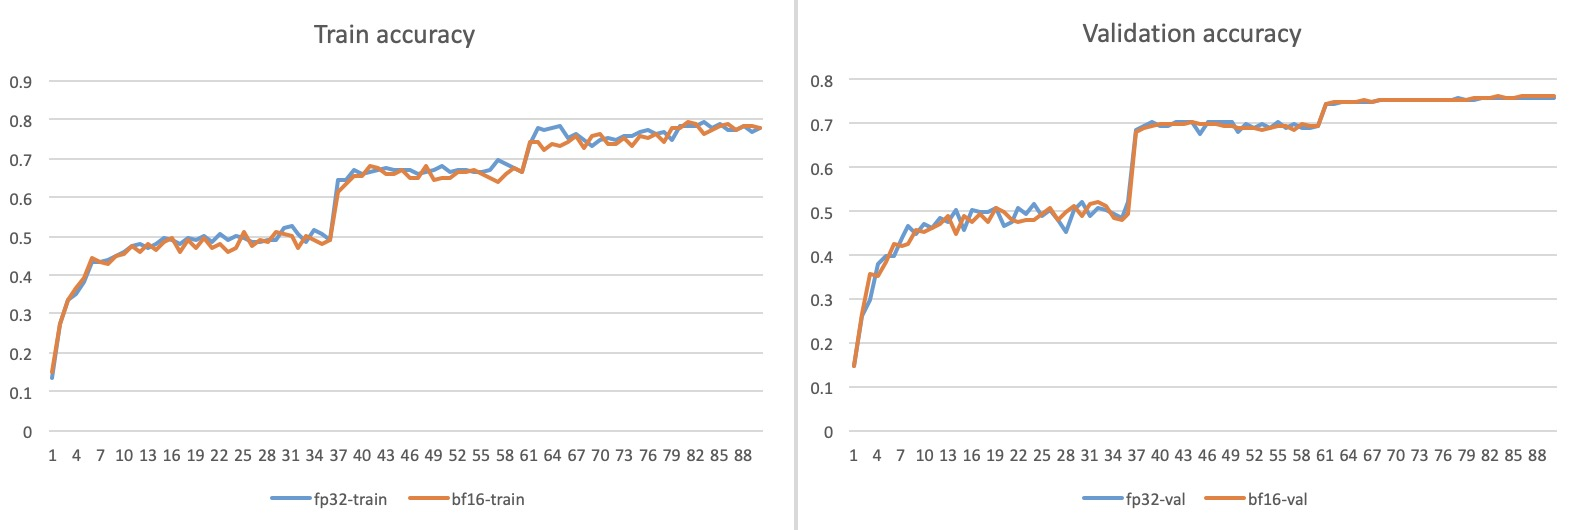
\includegraphics[width=13cm]{resnet50_4node_acc}
\caption{Resnet50中原始更新算法与LPDU算法收敛曲线}
\label{fig:resnet50_4node_acc}
\end{figure}

\begin{table}[htbp]
\centering
\begin{minipage}[t]{0.9\linewidth}
\caption{Resnet50在不同节点数下最终精度}
\label{tab:resnet50_diff_node_acc}
\begin{tabularx}{\linewidth}{l X X X }
\toprule[1.5pt]
{\song 数据集} & {\song 节点数} & {\song 原始更新算法(\%)} & {	\song LPDU算法(\%)}\\
\midrule[1pt]
ILSVRC2012 & 1 &  76.18 & 76.15\\
ILSVRC2012 & 4 & 76.20 & 75.98\\
ILSVRC2012 & 8 & 76.08 & 76.13\\
\bottomrule[1.5pt]
\end{tabularx}
\end{minipage}
\end{table}
为验证LPDU算法对神经网络的普遍适用性,本节以物体检测领域经典网络SSD为例,使用LPDU算法对其进行训练,通过比较原始更新算法与本文算法在验证集的收敛曲线和最终收敛结果验证LPDU算法的有效性。如图~\ref{fig:ssd_4node_acc}所示:在4节点8实例情况下,LPDU算法与原始更新算法在验证集上的mAP曲线基本重合,说明LPDU算法在物体检测网络中不会造成网络的精度损失。不同节点实例下原始更新算法与LPDU算法在VOC数据集上的最终结果如表~\ref{tab:ssd_diff_node_acc}所示,可知相同节点数下,LPDU算法与原始更新算法下验证集结果差距不超过0.4\%,在正常数据波动范围内。该误差来源于神经网络正常训练误差和BF16数据造成的部分数据损失。说明不同节点情况下LPDU算法均能保证神经网络的训练精度收敛到原始FP32更新算法相接近的精度,验证了LPDU算法的有效性与正确性。 

\begin{figure}[htp]
\centering
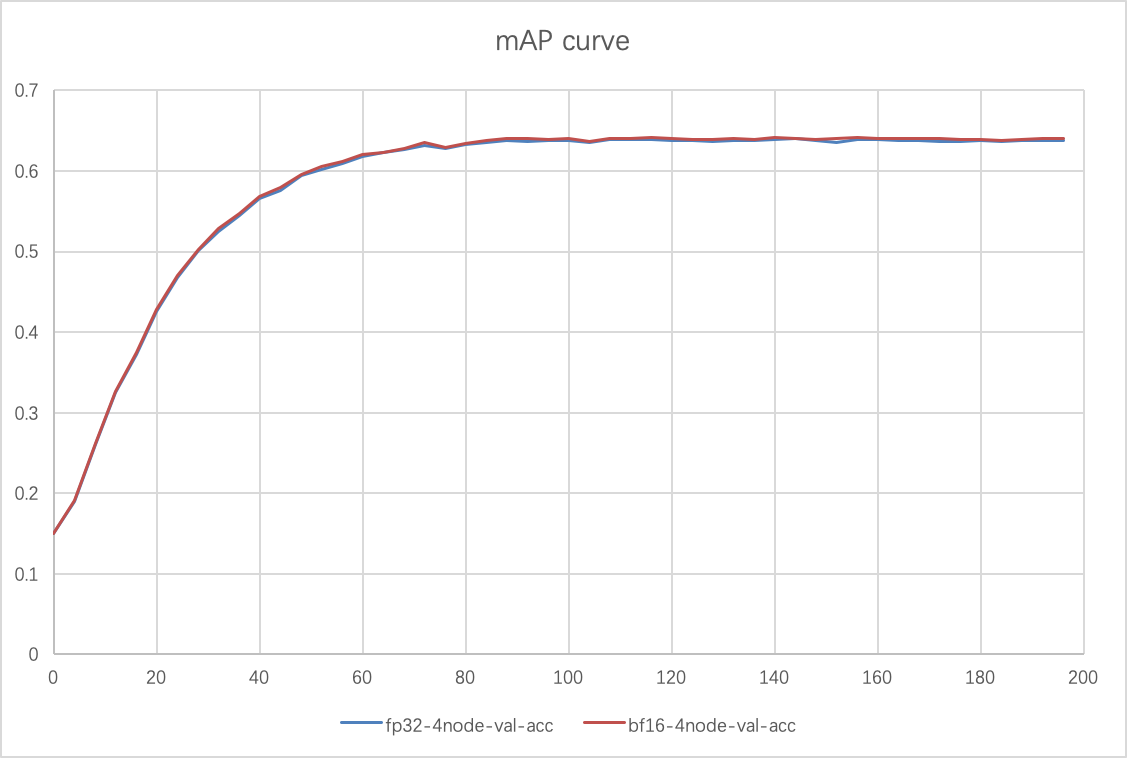
\includegraphics[width=10cm]{ssd_4node_acc}
\caption{SSD中原始更新算法与LPDU算法收敛曲线}
\label{fig:ssd_4node_acc}
\end{figure}


\begin{table}[htbp]
\centering
\begin{minipage}[t]{0.9\linewidth}
\caption{ssd在不同节点数下最终精度}
\label{tab:ssd_diff_node_acc}
\begin{tabularx}{\linewidth}{l X X X }
\toprule[1.5pt]
{\song 数据集} & {\song 节点数} & {\song 原始更新算法(\%)} & {	\song LPDU算法(\%)}\\
\midrule[1pt]
VOC2007+2012 & 1 & 64.22 & 64.18\\
VOC2007+2012 & 4 & 64.00 & 64.06\\
VOC2007+2012 & 8 & 64.04 & 63.64\\
\bottomrule[1.5pt]
\end{tabularx}
\end{minipage}
\end{table}

\section{小结}
本节通过比较LPDU算法与原始更新算法的训练效率与神经网络最终的收敛精度,说明了本章算法在不影响神经网络训练精度情况下,使得分布式训练效率有明显提升。也说明了LPDU算法对神经网络的普遍适用性。

\chapter{总结}
本文针对神经网络特点,提出低精度分布式更新算法,通过LPDC算法减少同步通信量减小同步开销,提升分布式训练效率。同时为避免低精度数据对网络模型造成影响使用MPU更新算法进行更新,从而保证神经网络训练精度与原始训练精度相一致。实验表明LPDU算法在不影响神经网络训练精度的情况下,能够有效提高分布式训练效率,且适用于目前主流的深度学习任务。
